
\section{Model Analysis}

\subsection{Pareto points}

\begin{figure}
	\centering
	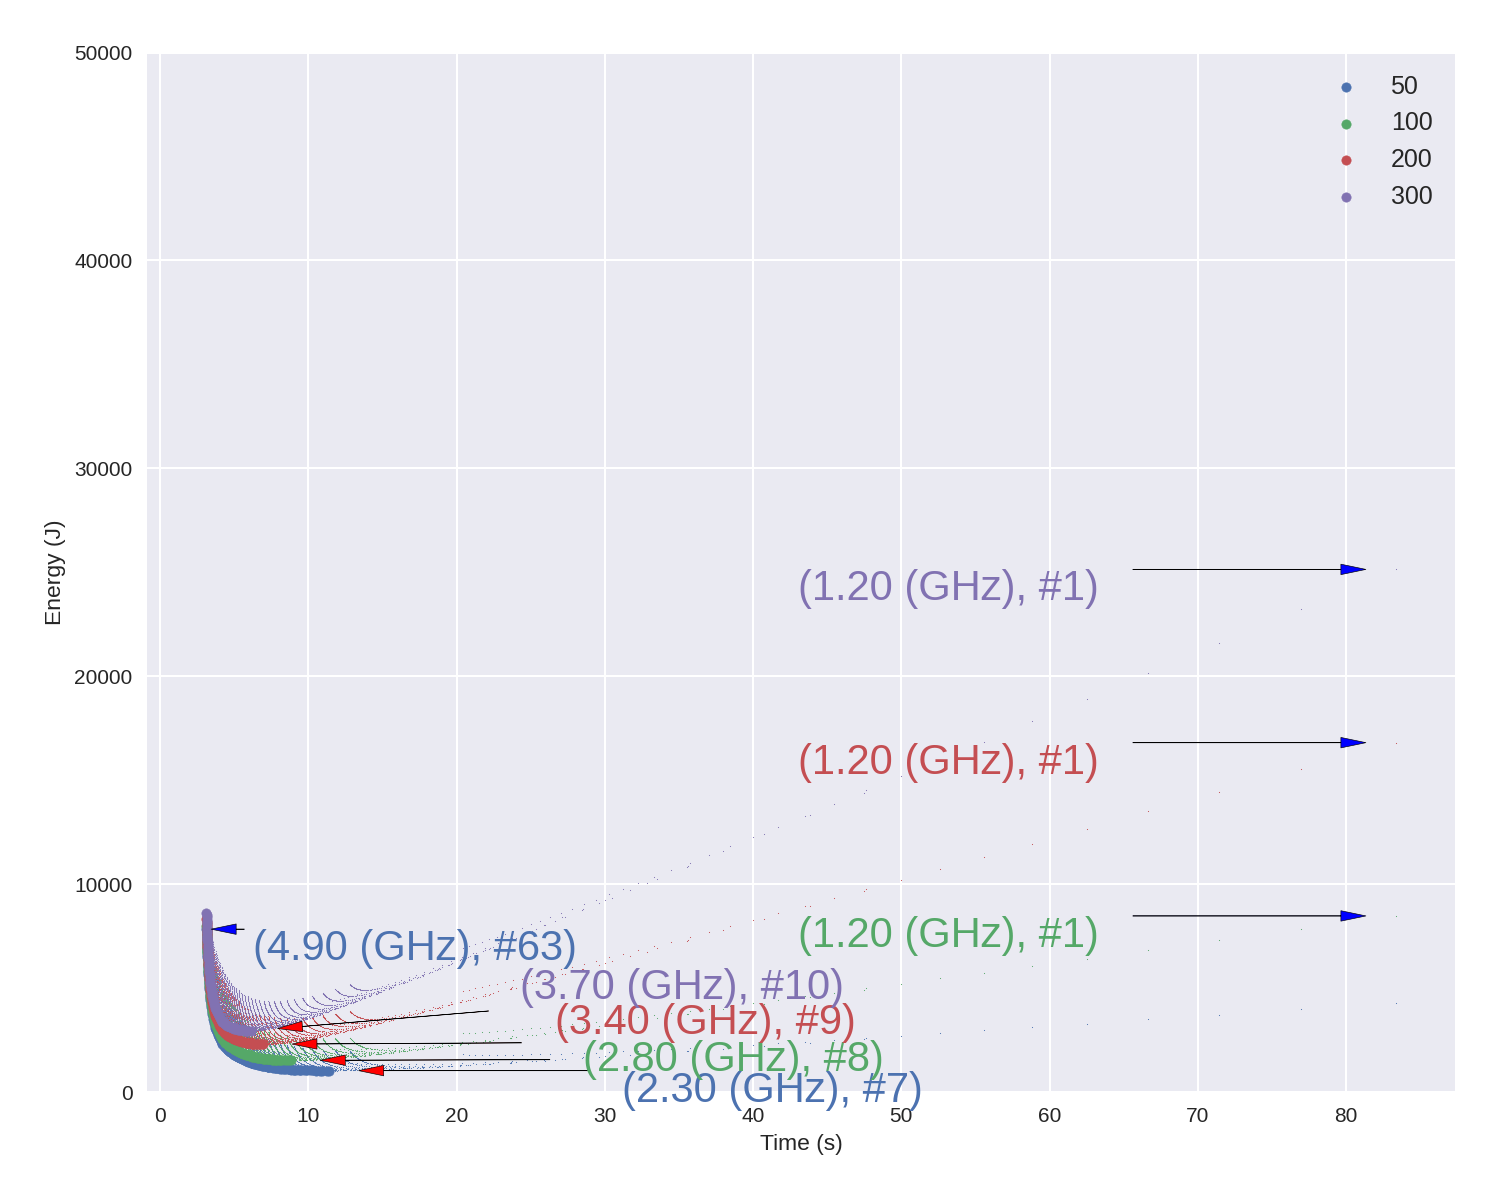
\includegraphics[width=\columnwidth]{models/figures/analisys/pareto_static_high.png}
	\caption{Pareto static energy}
	\label{fig:pareto_static_h}
\end{figure}


\begin{figure}
	\centering
	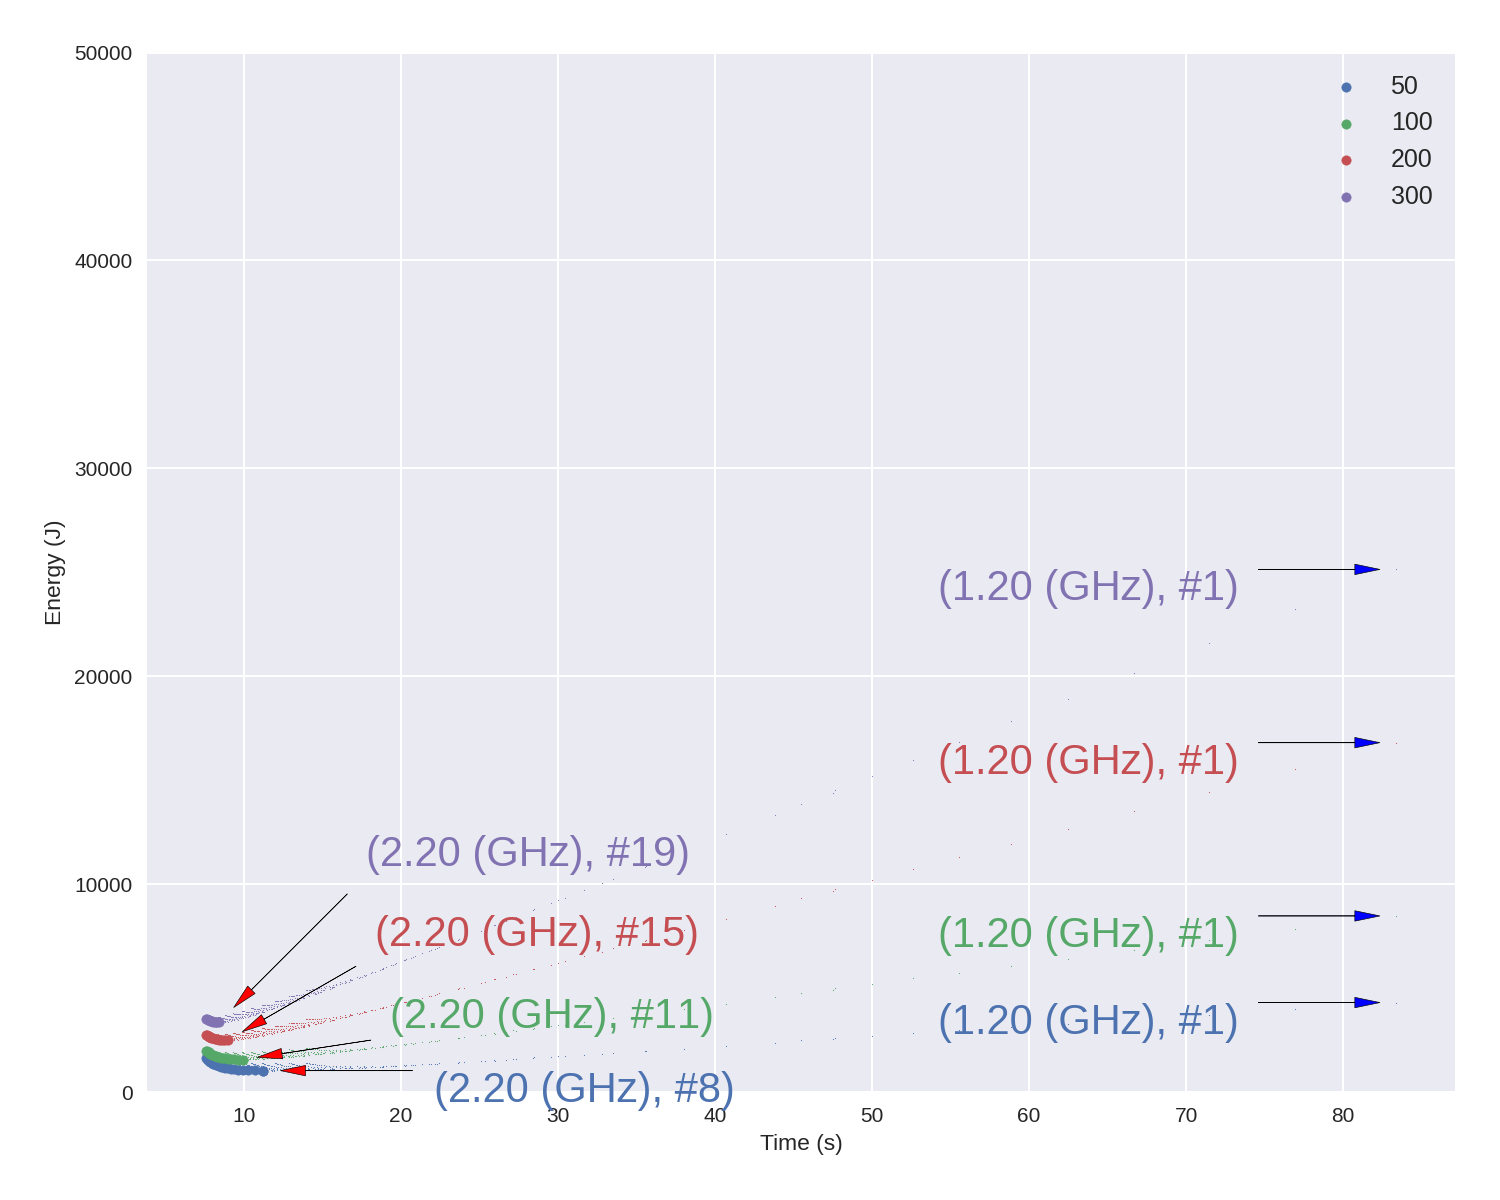
\includegraphics[width=\columnwidth]{models/figures/analisys/pareto_static_low.png}
	\caption{Pareto static energy}
	\label{fig:pareto_static_l}
\end{figure}


\begin{figure}
	\centering
	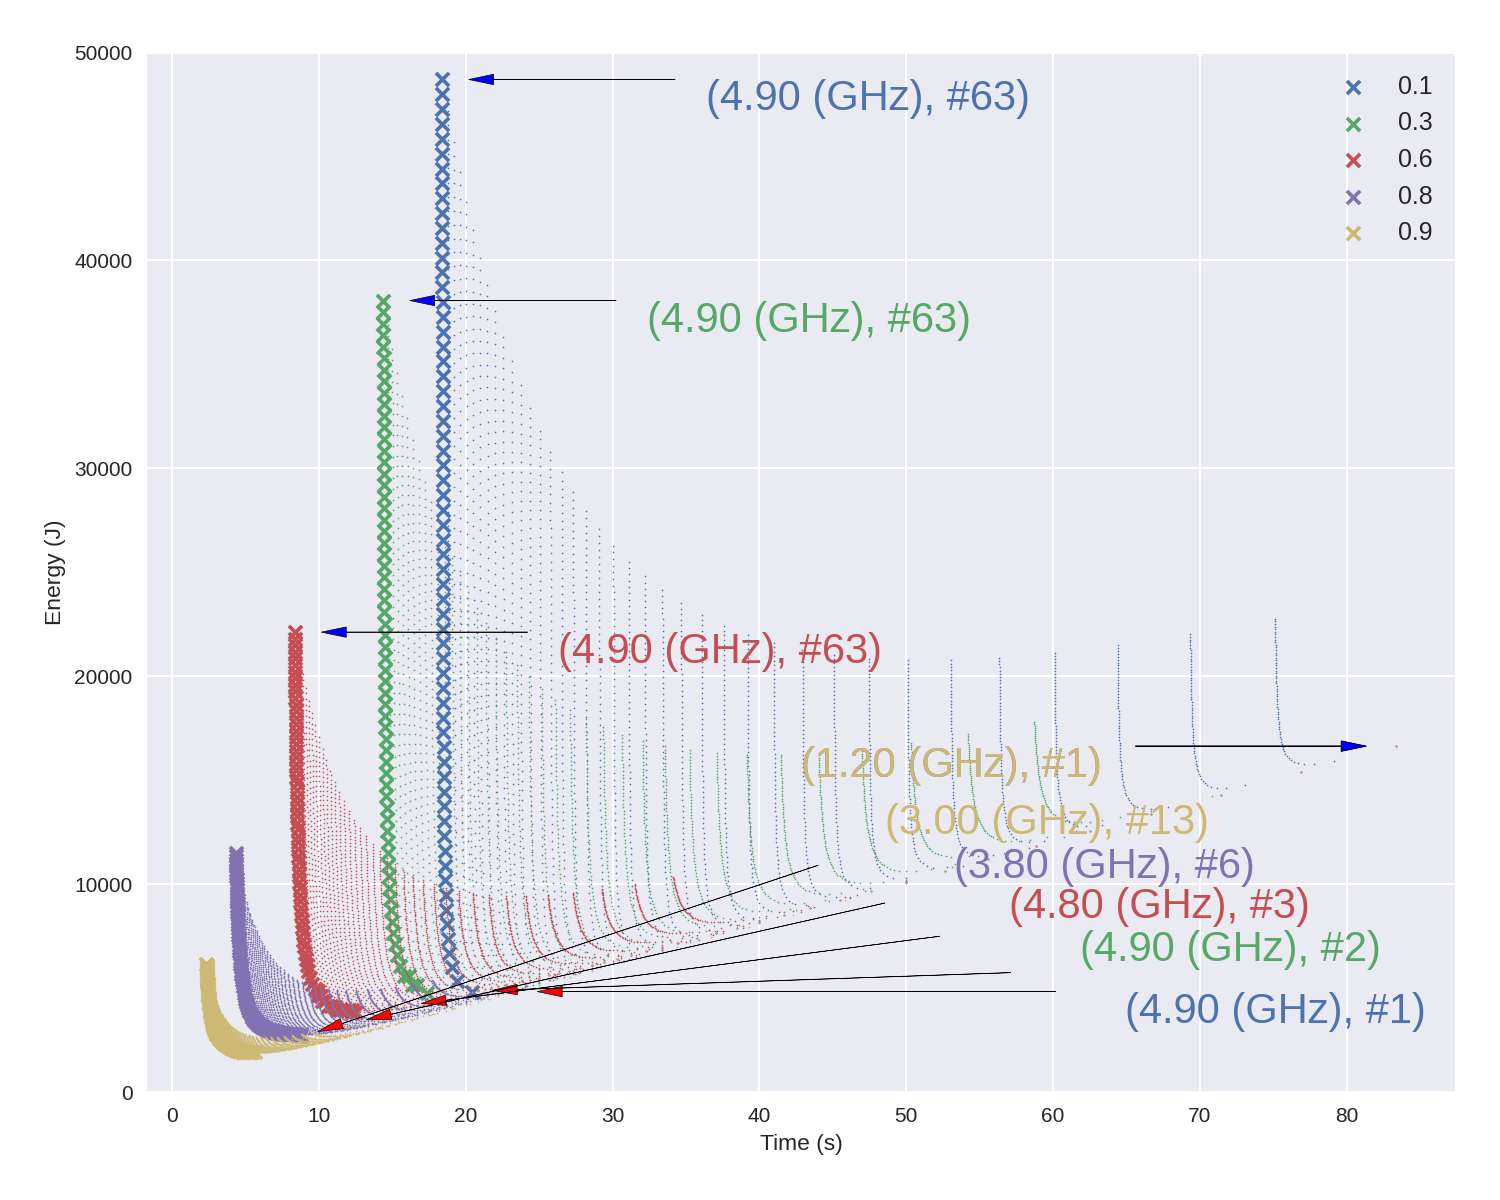
\includegraphics[width=\columnwidth]{models/figures/analisys/pareto_w_high.png}
	\caption{Pareto w energy}
	\label{fig:pareto_w_h}
\end{figure}

\begin{figure}
	\centering
	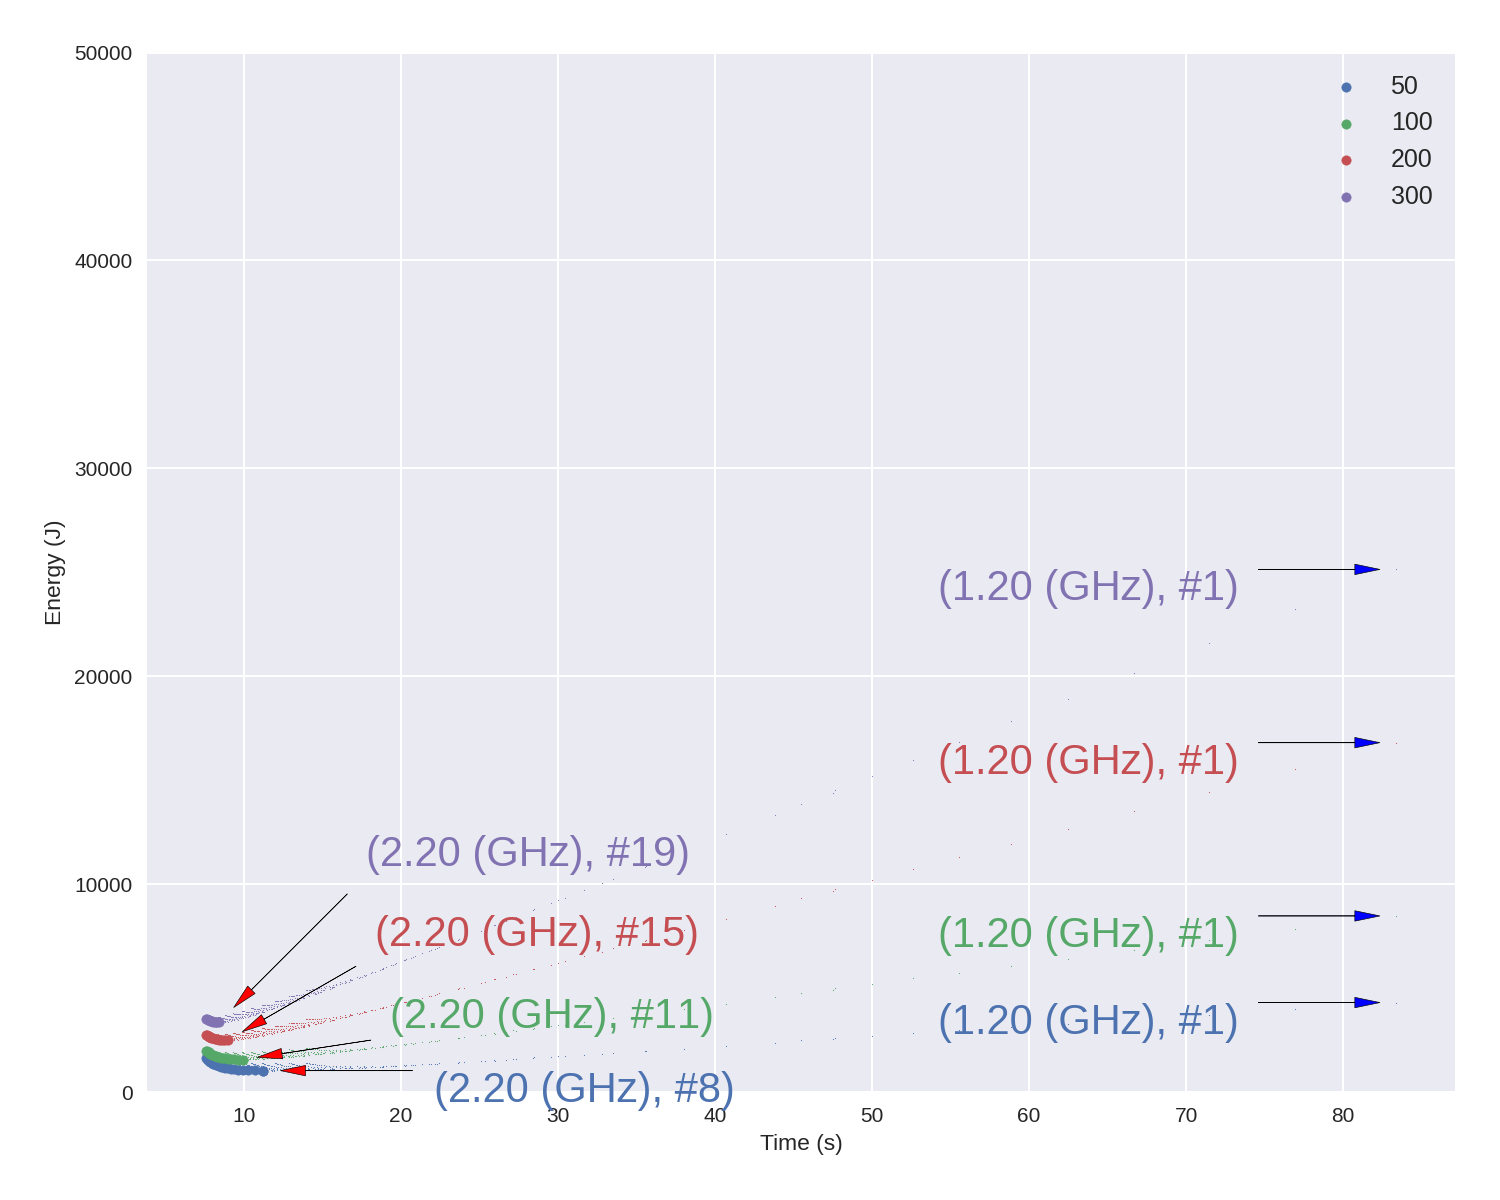
\includegraphics[width=\columnwidth]{models/figures/analisys/pareto_static_low.png}
	\caption{Pareto w energy}
	\label{fig:pareto_w_l}
\end{figure}

\subsection{Optimization under constraints}

\subsection{Gradient}

\begin{figure}[H]
	\centering
	\begin{subfigure}[b]{0.45\textwidth}
		\includegraphics[width=\textwidth]{ch5/image182}
	\end{subfigure}
	%
	\begin{subfigure}[b]{0.45\textwidth}
		\includegraphics[width=\textwidth]{ch5/image181}
	\end{subfigure}
\end{figure}

\begin{figure}[H]
	\centering
	\begin{subfigure}[b]{0.45\textwidth}
		\includegraphics[width=\textwidth]{ch5/image184}
	\end{subfigure}
	%
	\begin{subfigure}[b]{0.45\textwidth}
		\includegraphics[width=\textwidth]{ch5/image183}
	\end{subfigure}
\end{figure}

\begin{figure}[H]
	\centering
	\begin{subfigure}[b]{0.45\textwidth}
		\includegraphics[width=\textwidth]{ch5/image186}
	\end{subfigure}
	%
	\begin{subfigure}[b]{0.45\textwidth}
		\includegraphics[width=\textwidth]{ch5/image185}
	\end{subfigure}
\end{figure}

\begin{figure}[H]
	\centering
	\begin{subfigure}[b]{0.45\textwidth}
		\includegraphics[width=\textwidth]{ch5/image188}
	\end{subfigure}
	%
	\begin{subfigure}[b]{0.45\textwidth}
		\includegraphics[width=\textwidth]{ch5/image187}
	\end{subfigure}
\end{figure}

\begin{figure}[H]
	\centering
	\begin{subfigure}[b]{0.45\textwidth}
		\includegraphics[width=\textwidth]{ch5/image198}
	\end{subfigure}
	%
	\begin{subfigure}[b]{0.45\textwidth}
		\includegraphics[width=\textwidth]{ch5/image197}
	\end{subfigure}
\end{figure}

\begin{figure}[H]
	\centering
	\begin{subfigure}[b]{0.45\textwidth}
		\includegraphics[width=\textwidth]{ch5/image200}
	\end{subfigure}
	%
	\begin{subfigure}[b]{0.45\textwidth}
		\includegraphics[width=\textwidth]{ch5/image199}
	\end{subfigure}
\end{figure}

\begin{figure}[H]
	\centering
	\begin{subfigure}[b]{0.45\textwidth}
		\includegraphics[width=\textwidth]{ch5/image202}
	\end{subfigure}
	%
	\begin{subfigure}[b]{0.45\textwidth}
		\includegraphics[width=\textwidth]{ch5/image201}
	\end{subfigure}
\end{figure}

\begin{figure}[H]
	\centering
	\begin{subfigure}[b]{0.45\textwidth}
		\includegraphics[width=\textwidth]{ch5/image204}
	\end{subfigure}
	%
	\begin{subfigure}[b]{0.45\textwidth}
		\includegraphics[width=\textwidth]{ch5/image203}
	\end{subfigure}
\end{figure}


\subsection{Countorns}

\begin{figure}[H]
	\centering
	\begin{subfigure}[b]{0.45\textwidth}
		\includegraphics[width=\textwidth]{ch5/image202}
	\end{subfigure}
	%
	\begin{subfigure}[b]{0.45\textwidth}
		\includegraphics[width=\textwidth]{ch5/image208}
	\end{subfigure}
\end{figure}

\begin{figure}[H]
	\centering
	\begin{subfigure}[b]{0.45\textwidth}
		\includegraphics[width=\textwidth]{ch5/image204}
	\end{subfigure}
	%
	\begin{subfigure}[b]{0.45\textwidth}
		\includegraphics[width=\textwidth]{ch5/image206}
	\end{subfigure}
\end{figure}

\begin{figure}[H]
	\centering
	\begin{subfigure}[b]{0.45\textwidth}
		\includegraphics[width=\textwidth]{ch5/image198}
	\end{subfigure}
	%
	\begin{subfigure}[b]{0.45\textwidth}
		\includegraphics[width=\textwidth]{ch5/image211}
	\end{subfigure}
\end{figure}

\begin{figure}[H]
	\centering
	\begin{subfigure}[b]{0.45\textwidth}
		\includegraphics[width=\textwidth]{ch5/image200}
	\end{subfigure}
	%
	\begin{subfigure}[b]{0.45\textwidth}
		\includegraphics[width=\textwidth]{ch5/image212}
	\end{subfigure}
\end{figure}

\begin{figure}[H]
	\centering
	\begin{subfigure}[b]{0.45\textwidth}
		\includegraphics[width=\textwidth]{ch5/image186}
	\end{subfigure}
	%
	\begin{subfigure}[b]{0.45\textwidth}
		\includegraphics[width=\textwidth]{ch5/image217}
	\end{subfigure}
\end{figure}

\begin{figure}[H]
	\centering
	\begin{subfigure}[b]{0.45\textwidth}
		\includegraphics[width=\textwidth]{ch5/image188}
	\end{subfigure}
	%
	\begin{subfigure}[b]{0.45\textwidth}
		\includegraphics[width=\textwidth]{ch5/image218}
	\end{subfigure}
\end{figure}

\begin{figure}[H]
	\centering
	\begin{subfigure}[b]{0.45\textwidth}
		\includegraphics[width=\textwidth]{ch5/image182}
	\end{subfigure}
	%
	\begin{subfigure}[b]{0.45\textwidth}
		\includegraphics[width=\textwidth]{ch5/image219}
	\end{subfigure}
\end{figure}

\begin{figure}[H]
	\centering
	\begin{subfigure}[b]{0.45\textwidth}
		\includegraphics[width=\textwidth]{ch5/image184}
	\end{subfigure}
	%
	\begin{subfigure}[b]{0.45\textwidth}
		\includegraphics[width=\textwidth]{ch5/image220}
	\end{subfigure}
\end{figure}

